\Section{Script}

Script is the name of the programming language used in Bitcoin and its derivatives. It was not used to write the Bitcoin implementation but rather it is what makes transactions in Bitcoin so versatile. This section however will not focus on where or how Bitcoin uses Script, but rather on how Script itself functions.

Script is a forth-like stack based language that is not turing-complete.\cite{script_wiki}\cite{antonopoulos_2017} Turing-completeness means that a language can do anything that the imaginary turing-machine could do, in other words it basically means is that the language can do any mathematically sound operation. Script is \textbf{NOT} turing-complete on purpose, a good example is loops, in most languages there is some sort of structure that allows for a piece of code being executed repeatedly. In Scipt this is strictly disallowed, as it has neither for-loops or while-loops. This means that any given script will execute within a well defined deterministic time-span, and can never go on forever.

As mentioned earlier. Script is a stack-based language. That means that as the language executes it uses a stack to store data and variables. Do not confuse the term with the heap and stack from regular programming language discourse. In script there is no heap, instead the stack is the only form of memory, and it acts just as you would expect from a stack, to add a value you have to push it to the stack and to read a value you have to pop it from the stack.\cite{script_wiki}\cite{antonopoulos_2017}

The language itself is quite basic. It relies on operation codes (op codes) the size of a single byte. Most operations pop values from the stack, does something with the values, then pushes the result back on the stack. When Script is written out on paper many op codes and values are excluded, because they are implicit. For example: 

\texttt{OP\_PUSHDATA1 4 FFFFFFFF} 

This operation pushes 4 bytes to the stack, the bytes have the hexadecimal value \texttt{FFFFFFFF}. But usually when this operation is written out it is shorten to just:

\texttt{FFFFFFFF} 

\textbf{Whenever a hexadecimal value appears in the code it is implicit that that value is pushed to the stack in the form of bytes}. Here is another program:

\texttt{4 5 OP\_ADD 9 OP\_EQUAL}

This simple program will push 4 and 5 to the stack, \texttt{OP\_ADD}\cite{script_wiki} pops two values from the stack (4 and 5) adds them together and pushes the result back on the stack. Then a 9 is pushed to the stack. \texttt{OP\_EQUAL}\cite{script_wiki} pops two values form the stack and pushes a 1 if they were equal, 0 otherwise. In this case a 1 will be left on the stack as $4 + 5 = 9$. Figure \ref{fig:script} visualizes what happens at each step of execution.
\\
\begin{figure}[H]
	\centering
	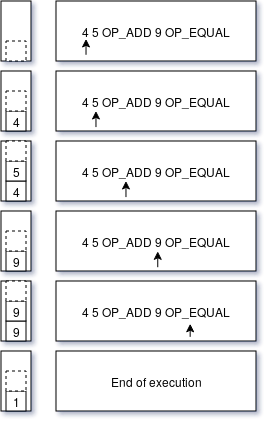
\includegraphics[width=0.4\textwidth]{background/images/script.png}
	\caption{Execution of simple program, to the left is the stack, to the right is the program with execution pointer}
	\label{fig:script}
\end{figure}

\Subsection{Complex operations}

There are some operations in Script with slightly higher complexity, which do not act like the others. One of them is \texttt{OP\_VERIFY}, this will perform a verify check on the script. It will pop one value from the stack, and if that value equates to false execution will end immidietly and the entire script will be marked as invalid (see section \ref{script_valid}).\cite{antonopoulos_2017}\cite{script_wiki} If the value equals true execution will continue where it left off. Some operations are combinations with the verify check, like for example \texttt{OP\_EQUALVERIFY}. This is equal to writing \texttt{OP\_EQUAL OP\_VERIFY}, meaning that it first does an equal check then verifys the result. There are other cases where the verify op-code is combined with other instructions.

\vspace{7mm}
\InsertBoxR{0}{
	\footnotesize\setlength\fboxsep{10pt}\setlength\fboxrule{1pt}
	\fcolorbox{IndianRed3}{SlateGray1}{\begin{minipage}{2.1in}
			\subsection*{Bug in Script}
			An interesting bit of trivia is that there is a bug in the language implementation. More specifically with the operation \texttt{OP\_CHECKMULTISIG}. The bug makes it so this operation pops one more value from the stack than it is supposed to. This was not discovered until the network had been running for a while. It can not be easily fixed as it is now a part of the consensus rules. All implementations of Bitcoin node has to implement the bugged version of this op code otherwise consensus on the validity of transactions will break.
			A fix to this bug would require a hardfok, see section \ref{soft_hard_fork}, so far it has not been done as it is considered to be not worth the time and effort.
	\end{minipage}}
}[9]

There are several operations for checking signatures. These are not so complex in terms of what they do in the script. Their implementation is quite complex however. They rely on outside information that is not present in the script to check the validity of a signature.\cite{script_wiki}\cite{antonopoulos_2017} The two most used are \texttt{OP\_CHECKSIG} and \texttt{OP\_CHECKMULTISIG}. These will not be covered in full in this section as they are more related to transactions so see section \ref{transactions} for a full explanation. 

\Subsection{Valid and invalid scripts}\label{script_valid}
At the end of execution a script is marked as either \\valid or invalid. A script is invalid for the following \\reasons\cite{antonopoulos_2017}:

\begin{itemize}
	\item The stack is empty
	\item There are more than one values on the stack
	\item The only value on the stack equates to false
	\item A VERIFY check fails sometime during execution.
\end{itemize}

A script is valid if and only if there is one value on the stack, and it is not equal to false.
